% updated April 2002 by Antje Endemann
% Based on CVPR 07 and LNCS, with modifications by DAF, AZ and elle, 2008 and AA, 2010, and CC, 2011; TT, 2014; AAS, 2016; AAS, 2020

\documentclass[runningheads]{llncs}
\usepackage{graphicx}
\usepackage{comment}
\usepackage{amsmath,amssymb} % define this before the line numbering.
\usepackage{color}
\usepackage{times}
\usepackage{microtype}
\frenchspacing
\usepackage[colorlinks=true,linkcolor=blue]{hyperref}

% INITIAL SUBMISSION - The following two lines are NOT commented
% CAMERA READY - Comment OUT the following two lines
\usepackage{ruler}
\usepackage[width=122mm,left=12mm,paperwidth=146mm,height=193mm,top=12mm,paperheight=217mm]{geometry}



\begin{document}
% \renewcommand\thelinenumber{\color[rgb]{0.2,0.5,0.8}\normalfont\sffamily\scriptsize\arabic{linenumber}\color[rgb]{0,0,0}}
% \renewcommand\makeLineNumber {\hss\thelinenumber\ \hspace{6mm} \rlap{\hskip\textwidth\ \hspace{6.5mm}\thelinenumber}}
% \linenumbers
\pagestyle{headings}
\mainmatter

\def\ECCVSubNumber{3290}  % Insert your submission number here

\title{3D Reconstruction of Clothes using a Human Body Model and its Application to Image-based VTON} % Replace with your title

% INITIAL SUBMISSION 
%\begin{comment}
\titlerunning{ECCV-20 submission ID \ECCVSubNumber} 
\authorrunning{ECCV-20 submission ID \ECCVSubNumber} 
\author{Anonymous ECCV submission}
\institute{Paper ID \ECCVSubNumber}
%\end{comment}
%******************

% CAMERA READY SUBMISSION
\begin{comment}
\titlerunning{3D Reconstruction of Clothes ... VTON}
% If the paper title is too long for the running head, you can set
% an abbreviated paper title here
%
\author{Matiur Rahman Minar\inst{1}\orcidID{0000-0002-3128-2915} \and
Thai Thanh Tuan\inst{2,3}\orcidID{1111-2222-3333-4444} \and
Heejune Ahn\inst{3}\orcidID{2222--3333-4444-5555}  \and
Paul Rosin\inst{3}\orcidID{2222--3333-4444-5555}   \and
Yukun Lai\inst{3}\orcidID{2222--3333-4444-5555}  }
%
\authorrunning{F. Author et al.}
% First names are abbreviated in the running head.
% If there are more than two authors, 'et al.' is used.
%
\institute{Seoul National University of Science and Technology, Seoul  08544, South Korea \and
Cardiff University, Cardiff, 69121 Heidelberg, UK
\email{heejune@seoultech.ac.kr}\\
\url{http://www.springer.com/gp/computer-science/lncs}}
\end{comment}
%******************
\maketitle

\begin{abstract}

Image-based virtual try-on (VTON) has drawn increasing attraction for online apparel shopping, mainly because of not requiring 3D information of try-on clothes and target humans. However, the existing 2D algorithms, even utilizing the advanced non-rigid deformation algorithm, can not handle the 3D shape changes for the postures of target humans. In this study, we propose the 3D cloth reconstruction method using 3D human body model. The 3D model of try-on cloth can be more easily deformed when applied to the rest posed standards human model. Thereafter the pose and shape of cloth can be transferred to the ones of the target humans estimated from a 2D image. Finally, the deformed cloth model can be rendered and blended together with unchanged cloth and human parts. The experimental results with an open dataset shows the reconstructed cloth shapes are significantly more natural compared to the 2D imaged based deformation results, when the human pose and shape are estimated accurately.         

\keywords{3D Model, SMPL, 3D Reconstruction, Cloth deformation, Virtual Try-on}
\end{abstract}




\begin{figure*}[t]
   \centering
\begin{tabular}{cccccc}

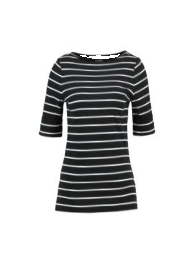
\includegraphics[width=2cm]{figures/c2dw/000008_1.png}&
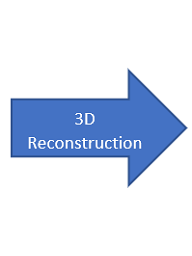
\includegraphics[width=2cm]{figures/arrow_recon.png}&
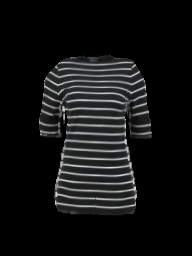
\includegraphics[width=2cm]{figures/c3drecon/000008_1_000303_0.png}&
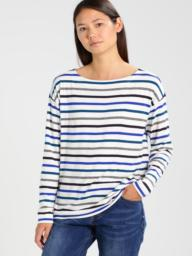
\includegraphics[width=2cm]{figures/image/000303_0.jpg}&
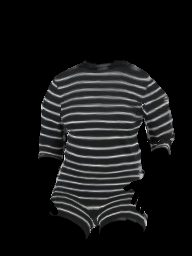
\includegraphics[width=2cm]{figures/c3dwfull/000008_1_000303_0.png}&
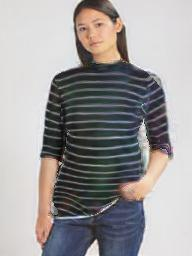
\includegraphics[width=2cm]{figures/try-on/000008_1_000303_0.jpg}\\


\includegraphics[width=2cm]{figures/c2dw/000005_1.png}&
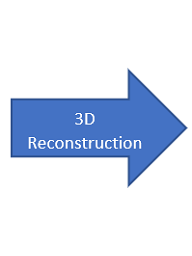
\includegraphics[width=2cm]{figures/arrow_recon.png}&
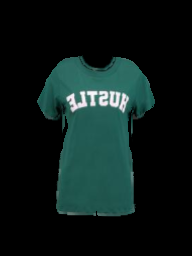
\includegraphics[width=2cm]{figures/c3drecon/000005_1_000303_0.png}&
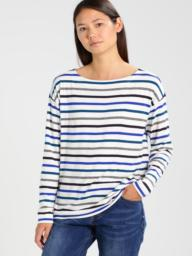
\includegraphics[width=2cm]{figures/image/000303_0.jpg}&

\includegraphics[width=2cm]{figures/c3dwfull/000005_1_000303_0.png}&

\includegraphics[width=2cm]{figures/try-on/000005_1_000303_0.jpg}\\

  Cloth input(2D)&&Cloth(3D)&Target&Cloth(Warped)&Try-on\\

\end{tabular}

    \caption{We reconstruct a 3D cloth model from single 2D cloth image. Then, given a target human image, we transfer the reconstructed 3D cloth model properties to the target human image, and render the warped cloth as in 3D deformed. Finally, we blend the rendered cloth into the target human and generate virtual try-on output image.}
    \label{fig:summary}
    
\end{figure*}



\section{Introduction} \label{section:intro}


Online fashion market has been growing rapidly every year. Unlike electronics, which makes it easy to standardize functions and performances, fashion apparels have infinite variations in style, forms, colors, texture, and materials.  Also the difference between personal preferences is huge. As a result, clothing purchasing decisions are very difficult to make with current non-customized information, like the cloth and models' try fit images. Therefore, virtual try-on (VTON) is a highly demanding technology for the online shopping. 

The early VTON technologies were based on 3D computer graphics technology that uses 3D models for a target human and clothing, which are usually expensive and difficult to obtain. Therefore, recently 2D image-based VTON technologies are being studied in academia and industry, fueled by the recent advances in computer vision technologies based on deep learning (DL). 

There have been many assumptions in problem settings from the general conditional human image generation related to virtual try-on applications. We consider the one with a try-on cloth and target human image is a practical condition which is assumed in many papers VITON\cite{Han2017VITONAI}, CP-VTON\cite{Wang2018TowardCI} , and the following  \cite{Sun2019ImageBasedVT,Yu_2019_ICCV}. Therefore, we also consider the virtual try-on problem that uses the try-on clothes and human images and generates a new synthetic image that the target human replaced the current top or bottom cloth with the try-on cloth. In this paper, we limit our application to top cloth only due to the restricted data set. However, we consider that the bottom, e.g. pants cases would be easier than top cloth cases.


\begin{figure}[t]
\centering
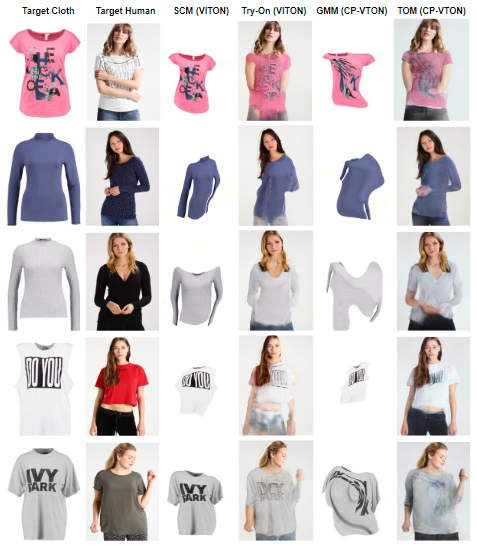
\includegraphics[scale=0.6]{figures/2dvton_diff.png}
\caption{Failures of image-based 2D cloth deformations for Virtual Try-On (Different clothes pairs)}
\label{fig:2dvtondiff}
\end{figure}


The existing 2D image-based algorithms seemingly generate high quality virtual try-on results. However, our classified analysis on the cloth styles, human poses, and shapes reveals significant problems, illustrated in Figure \ref{fig:2dvtondiff} and \ref{fig:classified2DVTONresult}. One reason of the seemingly high quality in the existing algorithms are mainly due to the low complexity of the dataset, i.e., most clothes are short-sleeved, and mono-colored, and the poses of humans are mild. Specifically, the results with the long-sleeved clothing arms and body posed show far low qualities than the presented results in the respective papers\cite{Han2017VITONAI,Wang2018TowardCI}. We identified 5 major issues in the state-of-the-art CP-VTON\cite{Wang2018TowardCI} pipeline, some of which are tackled in the following papers\cite{Sun2019ImageBasedVT,Yu_2019_ICCV}. Firstly, the target try-on area is dependent upon current cloth shape. Especially, the neck area pixels are labeled as background and some body areas are occluded by hairs or accessories, which affects in cloth warping and blending. Secondly, all unintended parts other than target clothing area, i.e., face, bottom-clothes and legs should be preserved in blending stage. However, other body parts except face and hairs are missing in CP-VTON\cite{Wang2018TowardCI} human representation inputs and generated at blending stage, which is all right for general synthesis application, but not desirable in virtual try-on application (Figure \ref{fig:2dvtondiff}, \ref{fig:classified2DVTONresult}). Thirdly, the texture is often not vivid, which is due to the composition. Examining the original loss function of Try-on Module (TOM) network, the term for the composition alpha mask are poorly formulated as in simple regularization loss.   

\begin{equation}
L = c_1 | I_0-I_{GT} |+  c_2 L_{VGG}+c_3 |1-M_0 |        
\end{equation} 

Fourthly, since no label in the area of warped cloth is the same color as background, white colored clothes are confused and improperly processed in the blending stage (Fig. \ref{fig:2dvtondiff} (c))
Finally, Geometric Matching Module (GMM) using Spatial Transformer Network\cite{JaderbergSZK15} with TPS (Thin Plate Spline)\cite{Bookstein1989PrincipalWT} deformation cannot handle strong 3D deformation due to the target pose, also  generates artifacts due to the person representation inputs. For example, hands-up and folded arms.  Note that many errors in the warping stage are often hidden in the blending stage, especially when the target clothes are single-colored, which can be expected in practical conditions (Figure \ref{fig:2dvtondiff}, \ref{fig:classified2DVTONresult}).

In this paper, we focus on the last but most difficult problems that cannot be solved in pure 2D image-based algorithm. The 3D cloth deformation is inherently difficult for 2D warping method, including non-rigid one, like TPS algorithm, we propose to first reconstruct 3D model of try-on cloth, then apply the pose and shape transfer for the target human, and finally blending with unchanged image contents like the face, bottom cloth, and background. Therefore, one of main the tasks now is to reconstruct 3D cloth model from 2D try-on cloth image. 3D clothed body model reconstruction have been studied in previous works \cite{natsume2019siclope,saito2019pifu}, however it still needs significant improvements for general condition. Our key idea in this step is that, once we can control the human pose and body shape to become similar to the try-on cloth's, the 3D reconstruction process can be made much easier, and the reconstruction quality would be much higher than general pose and shape condition. Figure \ref{fig:summary} shows a summarized glimpse of our total approach.

Therefore, in the Section \ref{section:3dclothrecon}, we describe the 3D cloth reconstruction algorithm. We divide the reconstruction step into 2D matching of cloth to the standard body silhouette and the 3D reconstruction of cloth. The later 3D reconstruction step is done through the SMPLify\cite{Bogo2016SMPLify} algorithm for the SMPL 3D body model\cite{Loper2015SMPLAS}.  In Section \ref{section:clothtransfer}, we describe the blending method, where the 3D cloth models are transferred to the target human images, through SMPL body parameters of shapes and poses. Then the transferred 3D reconstructed cloth is rendered and blended to the target human image. In this step, we reused the 2D virtual try-on blending algorithm with the modification for the condition.  The sampled results from dataset are presented in Section \ref{section:clothtransfer} and the paper is concluded in Section \ref{section:conclusion}. In addition to our main study, we added the classified quality evaluation of the previous 2D image based virtual try-on algorithms for the completeness of the paper.


  % intro
\section{Classified Image Based Performance Evaluation}

\subsection{Image-based VTON}

In this Section, we start with evaluating the 2D image-based virtual try-on (VTON) algorithms. We consider CP-VTON\cite{Wang2018TowardCI} published in 2018 as the benchmark algorithm. Most of the recently proposed image-based approaches\cite{Han2017VITONAI,Sun2019ImageBasedVT,Yu_2019_ICCV} share same input images and information conditions as CP-VTON and compare the results with it. Here we include the Shape-Context Matching (SCM) based-VTON, VITON\cite{Han2017VITONAI}, and  CP-VTON\cite{Wang2018TowardCI}, however, we believe the performance strengths and weaknesses are similar in the other algorithms as well.


The Image based virtual try-on algorithms are mostly composed of two stages: (1) cloth warping step that warps the try-on cloth to align with the pose and shape of the target model (called GMM in CP-VTON: geometric Matching Module)\cite{Wang2018TowardCI}, and (2) blending step that blends the warped cloth onto the target human image (called TON in CP-VTON: Try-On Network)\cite{Wang2018TowardCI}. CP-VTON assumes the target human image is pre-processed for a cloth agnostic human representation by a human pose estimation like OpenPose\cite{Cao2018OpenPoseRM} and human parsing like LIP\cite{Liang2018LookIP}. The human representation is composed of 1) heat maps for each joints 2) silhouette of human body, and 3) face and skin pixels patches (non-cloth and human identity area). We use the same dataset collected by Han et al. used in VITON\cite{Han2017VITONAI} and CP-VTON\cite{Wang2018TowardCI} papers.
 

\subsection{Classified quality}

Even though the success and failure cases are presented and compared with other algorithms' results, the failure case analysis is not enough for understanding the origin of failure cases and therefore difficult to find the solution for them. A classified evaluation would be better for this understanding. Here we summarized the classified results from our another study. We classify input try-on cloth and target human images according to the posture and body type of the person, the degree of occlusion of the clothes, and the characteristics of the clothes. Quality is compared in IoU for the warping step and in SSIM for the final blending step for same cloth re-try-on cases. We also tested for the new cloth try-on cases but did not include here for limitation of spaces, and the same cloth cases are enough to explain the tendencies of the performances. Though in general CP-VTON generates the best quality image, the relative comparison is not the main purpose of the analysis. Please refer to Figure \ref{fig:classified2DVTONresult} for detailed results.


\begin{figure}[t]
\centering
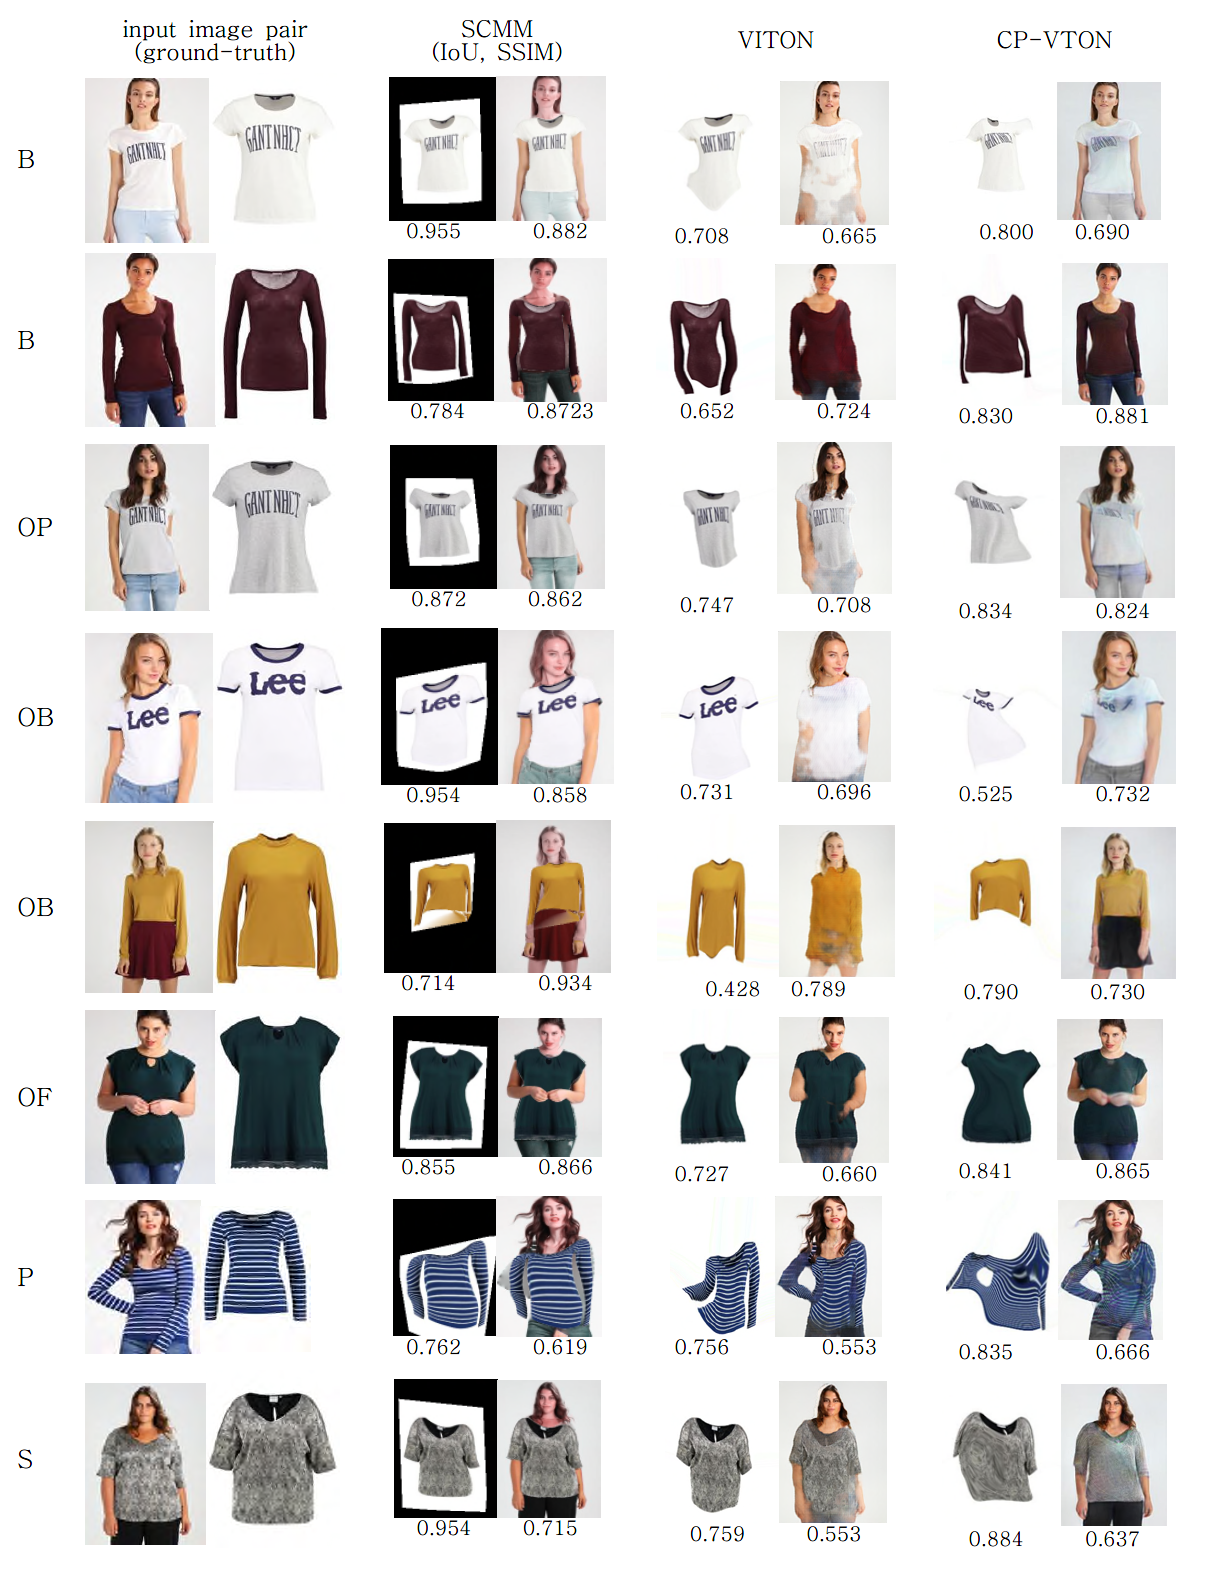
\includegraphics[height=13.5cm, scale=1]{figures/2dvton_same.png}   % TODO
\caption{Classified VTON result: same clothes}
\label{fig:classified2DVTONresult}
\end{figure}



////

Here I will describe the evaluation discussion, finally commenting that the GMM has serious problem.

////

Especially note that the warped cloth are often too much different for desired shape. It is originated two facts. First the 3D deformation that any 2D deformation including non-rigid transform such as TPS is quite limited, especially any 2D deformation cannot handle when the two area in the original image are overlapped in the destination images. There for when the arms of long sleeved cloth occlude the main body, 2D warping cannot approximate the 3D deformation properly. Second, the deformation needs corresponding points  between the source nd target image. The cloth are extremely difficult object to find the corresponding points. The STN (spatial transform network)\cite{JaderbergSZK15} and SCM (shape context matching)\cite{BelongieMP02} cannot find the corresponding points when the target cloth and original cloth has different shapes. In conclusion, the 2D image based algorithm has serious limitation in the range of applications. It can apply to the mild posed target human only and simple short sleeved cloth, mainly because the inherent limitation of 2D deformation method including non-rigid ones, and the poor performance of matching algorithm.  To overcome this limitation, we consider to model the try-on cloth into 3D model and apply the 3D deformation


  % performance evaluation
\section{3D model reconstruction of cloth} \label{section:3dclothrecon}

\subsection{Overview} 

For 3D human body model, we use Skinned Multi-Person Linear model (SMPL)\cite{Loper2015SMPLAS}, because SMPL has well defined control variables for shape and pose, and well defined parameter estimation algorithms as well. For similar reasons, SMPL\cite{Loper2015SMPLAS} model have been utilized in many research works \cite{Zanfir2018HumanAT,Weng2018PhotoW3}. Furthermore, since it is based on blend skinning, SMPL is compatible with existing rendering engines\cite{Loper2015SMPLAS} and made available for research purposes. SMPL is a skinned vertex-based model that accurately represents a wide variety of body shapes in natural human poses. The parameters of the model are learned from data including the rest pose template, blend weights, pose-dependent blend shapes, identity-dependent blend shapes, and a regressor from vertices to joint locations. Unlike previous models, the pose-dependent blend shapes are a linear function of the elements of the pose rotation matrices. This simple formulation enables training the entire model from a relatively large number of aligned 3D meshes of different people in different poses. \cite{Loper2015SMPLAS} 


\begin{figure}[t]
\centering
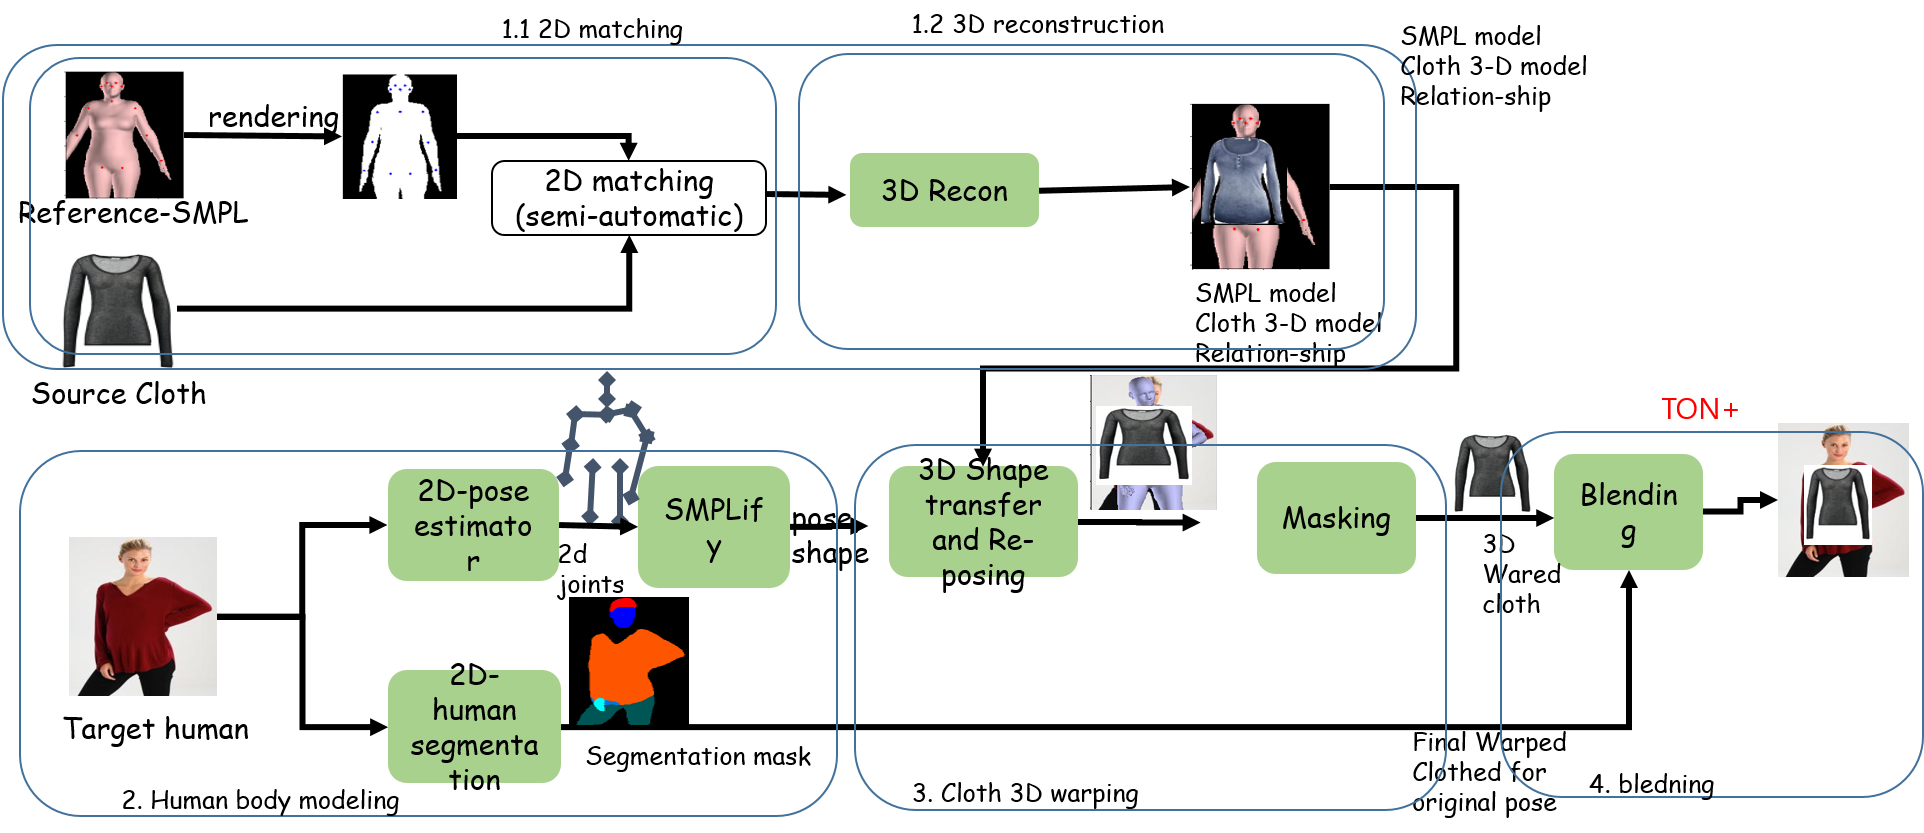
\includegraphics[height=4.5cm, scale=1]{figures/pipeline.png}   % TODO
\caption{Pipeline}
\label{fig:piepline}
\end{figure}


For estimating the SMPL\cite{Loper2015SMPLAS} parameters, we use SMPLify\cite{Bogo2016SMPLify} method in this study. However, any other methods can be used since we assume nothing on the procedure and use estimated parameters only. SMPLify\cite{Bogo2016SMPLify} uses 2D human body joint information often obtained from deep learning based method like DeepCut\cite{pishchulin2016deepcut} or OpenPose\cite{Cao2018OpenPoseRM}, and minimize the projected joint locations and the given (considered true) 2D joint locations. The cost function can include other priors and silhouette information. We made minor optimization for half body dataset, such as joint location mapping between the joints of used fashion data set and SMPLify joint definition, and conditional inclusion of invisible joints and initialization step.  From our experiments with all 2032 test images, we found that the SMPLify quality should be much improved for fully automatic application to VTON application. So the result included in this paper excluded the bad matching cases which is around 30\% of all test images.    
  
Clothed human reconstruction using 3D SMPL model\cite{Loper2015SMPLAS} have been studied in several previous works \cite{Weng2018PhotoW3,Zanfir2018HumanAT}. Although we are successful in modeling human body, there are further difficulties to recover the clothed human model from body model. It is due to the cloth vertices, which do not directly correspond to the human body's. Even if it does, it is still difficult to estimate the differences between two. Also, the textures of clothes can be occluded by other parts of clothes and human body parts. Previous works try to solve the problem in the given image condition. Therefore, the results are strongly dependent upon the input images. In this paper, we make this step easy by using simple standard human pose, where all frontal parts of clothes are well separated and visible. This setup cannot handle all problems in the clothed human model reconstruction, however, it can greatly make it easy. The following subsection describe the procedure in details.



\subsection{2D Standard Cloth matching}


To align the try-on cloth image with 3D SMPL\cite{Loper2015SMPLAS} body model, first their dimension spaces should be matched. Natural way would be first rendering the SMPL\cite{Loper2015SMPLAS} body model into 2D image space. However, as stated above, the matching between cloth image and body silhouette is not a simple task. For simplicity, we assume we can segment the silhouette, so that the remaining area can be easily matched by Shape-Context Matching (SCM)\cite{BelongieMP02} algorithm. We argue that, for virtual try-on commercial application, this step can be monitored by service provider side which is practically acceptable. The manual operation from the customer in the try-on step would not be acceptable in general service environment.   

\begin{equation}
(I_{c, warped}, M_{c, warped})  = T_{SMPL} ((I_c, M_c))
\end{equation}


\begin{figure}[t]
\centering
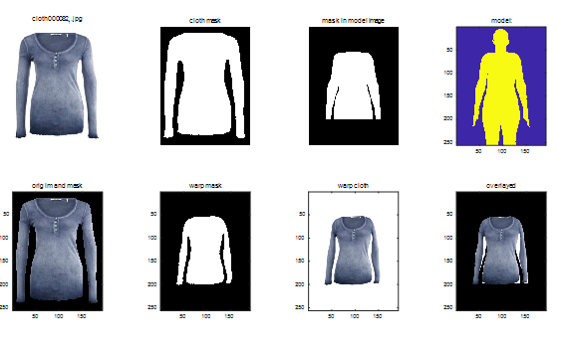
\includegraphics[width=9cm]{figures/2dmatching.png}   % TODO
\caption{2D matching between clothing image and 3D body model silhouette mask}
\label{fig:2DmatchingOfClothAndBody}
\end{figure}


\subsection{3D cloth model reconstruction }


The 3D reconstruction process from aligned cloth image and projected silhouette consists of 2 steps. First, the vertices of 3D body mesh are projected into 2D image space, the boundary vertices in 2D spaces, and the cloth boundaries are used for corresponding points. The corresponding points in the cloth boundary is defined as the closest points from the projected vertices. This step works well in our cases differently from Photo Wake-up\cite{Weng2018PhotoW3} study, because the part of body and cloth are not self-overlapped. This is a implementation benefits of our approach. From the corresponding point pairs, a This-Plate Spline (TPS)\cite{Bookstein1989PrincipalWT} parameters are estimated and applied to the mesh points. The new mesh points are considered as the vertices projected from 3D mesh of cloth. From 2D points to 3D points are done with inverse projection with depth obtained from the body with a small constant gap. In reality the gap between the cloth and body cannot be constant but it works with tight or simple clothes. Further research works are needed for accurate depth estimation.   


\begin{equation}
V_{clothed} = Pjt^{-1} ( T( (Pjt(V_{body})), depth(V_{body}) )
\end{equation}


The try-on cloth images are used as the texture for the 3D cloth mesh. We can filter the vertices corresponding to cloth and get the cloth 3D mesh model. Figure \ref{fig:3DreconstructedCloth} shows the reconstructed cloth examples. 


\begin{figure}[t]
\centering
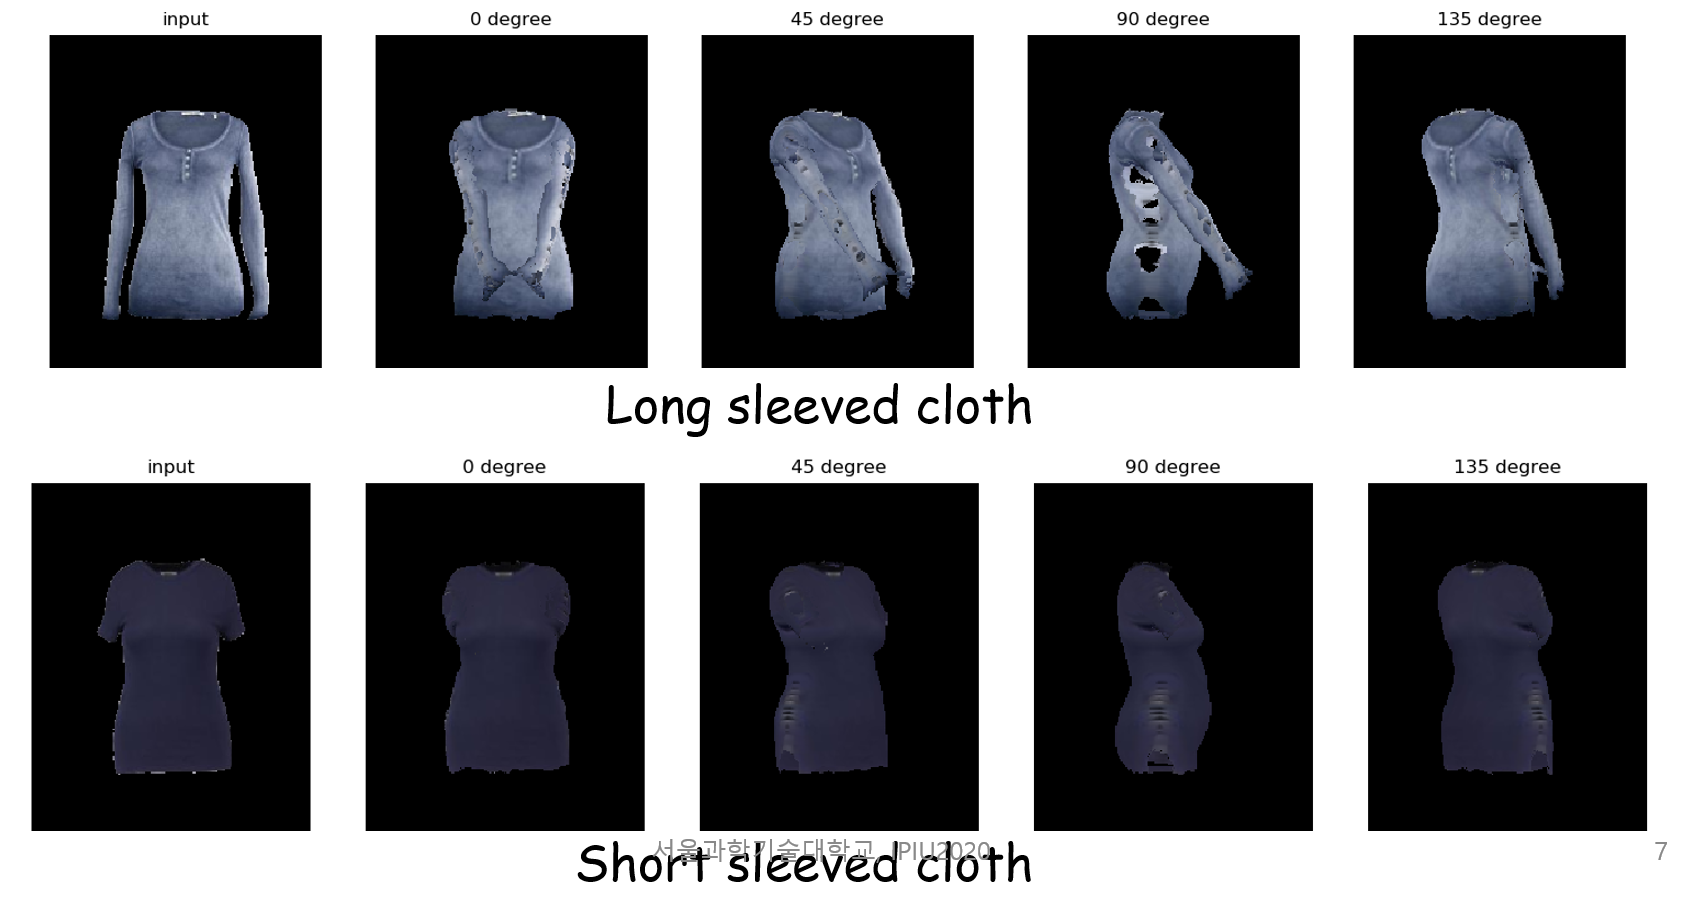
\includegraphics[height=6.5cm]{figures/3dclothrecon.png}   % TODO
\caption{3D reconstructed cloth}
\label{fig:3DreconstructedCloth}
\end{figure}



  % 3D reconstruction
\section{Transfer of 3D cloth model to the target Human and Virtual Try-On }  \label{section:clothtransfer}


\subsection{Transfer of 3D cloth model to the target Human} 

The 3D model and texture information obtained from 3D reconstruction (Section \ref{section:3dclothrecon}) are for the standard shape and posed person. To apply this information for virtual try-on application, we have to apply the shape and pose parameters of the target human image estimated from SMPLify\cite{Bogo2016SMPLify} step. Instead of applying the shape and pose parameters to the obtained clothed 3D model, we transfer the displacement of cloth vertices to the target human body model, since the application of new parameters to the body model provide much better natural results. (Figure \ref{fig:clothtransfertryon})


Multiple options can be considered for the transfer. We could transfer the physical size of cloth or keep the fit, i.e., keep the displacement from the body to cloth vertices as before.  We simply decide the fit-preserving option for showing more natural results for final fitting.  

Technically, the displacement should be calculated locally. First, we calculated the local coordinate at each vertices. We define the local coordinates: surface normal vector as z-axis, and the vector to smallest indexed edges as x-axis, and their cross product vector as y-axis as the following equations.


\begin{align}
 u_{z} =  normal(V_{body})  \\
 u_{x} = u^{''}_{x}/ |u^{''}_{x} |, 
 u^{''}_{x} = u^{'}_{x} - u^{'}_{x} \cdot u_{z}, 
 u^{'}_{x} = (V_{argmin(N_V) } - V_{body}) \\
 u_{y}  =  u_z \otimes u_x,
\end{align} 
 where $N_V$ is the neighbor vertex of $V$.
 

The displacement is expressed in the local coordinates and then used the same way in the new target body surfaces for location transfer.

\begin{equation}
\overrightarrow{d} = (d_x, d_y, d_z) = V_{clothed} - V_{body} \: in \: (u_x, u_y, u_z | V_{body})
\end{equation}


\begin{equation}
 V'_{clothed} = V'_{body} + \overrightarrow{d} \: in \: (u_x, u_y, u_z | V'_{body})
\end{equation}



\begin{figure*}
   \centering
\begin{tabular}{cccccccc}

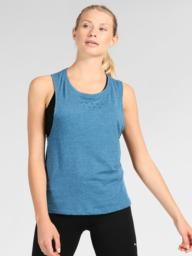
\includegraphics[width=1cm]{figures/image/001715_0.jpg}&
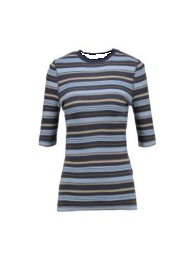
\includegraphics[width=1cm]{figures/c2dw/015077_1.png}&
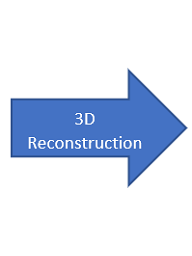
\includegraphics[width=1cm]{figures/arrow_recon.png}&
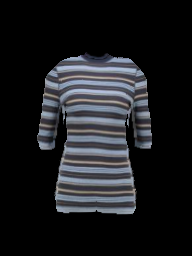
\includegraphics[width=1cm]{figures/c3drecon/015077_1_001715_0.png}&
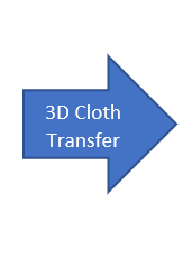
\includegraphics[width=1cm]{figures/arrow_transfer.png}&
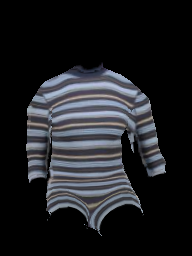
\includegraphics[width=1cm]{figures/c3dwfull/015077_1_001715_0.png}&
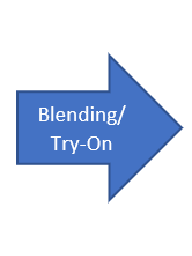
\includegraphics[width=1cm]{figures/arrow_blending.png}&
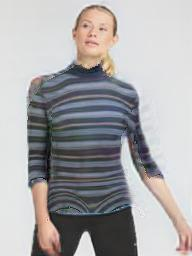
\includegraphics[width=1cm]{figures/try-on/015077_1_001715_0.jpg}\\

Target&Cloth(2D)&&Cloth(3D)&&Cloth(Warped)&&Try-on\\

\end{tabular}

    \caption{Transfer of 3D cloth model to the target Human and Virtual Try-On}
    \label{fig:clothtransfertryon}
    
\end{figure*}



\subsection{Blending of warped cloth with target human image}  \label{section:tryon}

For our experiment, we used an extended version of Try-on module (TOM) from CP-VTON\cite{Wang2018TowardCI}. We trained  our updated try-on module with the dataset collected by Han et al.\cite{Han2017VITONAI}, and used that trained network for testing with the 3D warped cloth (Figure \ref{fig:clothtransfertryon}). We updated 3 things from original Try-on module (TOM) of CP-VTON\cite{Wang2018TowardCI} for our implementation. Firstly, we included the un-intended body and clothing areas into the person representation input to Try-on module (TOM) network\cite{Wang2018TowardCI}. Secondly, we included the warped cloth mask into network inputs, so that it can differentiate the target cloth area regardless of cloth color. Thirdly, we updated the composite mask loss function\cite{Wang2018TowardCI}. In the mask loss term in Try-on module loss function\cite{Wang2018TowardCI}, we replaced the Composition Mask with supervised ground truth mask for a strong alpha mask.


\begin{equation}
L = \lambda_{L1} || I_0-I_{GT}||_1+  \lambda_{VGG} L_{VGG} + \lambda_{mask} ||M_{GT}-M_o||_1       
\end{equation}


However, using 3D warped clothes as in warped clothes inputs to try-on module network, do not provide highly satisfactory results as expected, compared to the qualities improved in the warped clothes. We assume that this is due to the mismatch in warped clothes, between training data inputs to our testing data inputs. Therefore, we think it would be better to train the blending network, i.e., the try-on module with 3D warped clothes, generated by our approach for further improvements. We may think of using other options as well. For instance, we can reconstruct all the clothed information from the target user and overlay the transferred cloth.






  % cloth transfer


\section{Conclusions}  \label{section:conclusion}

In this paper, we proposed 3D cloth model reconstruction method using single cloth image. Leveraging the 3D body model, we can make it easy to reconstruct 3D shape information. The 3D cloth model is used for transferring the cloth to target human model.  The transferred clothes can be integrated with the human image contents for realizing the pose and shape changes which can not be realizable by existing image based VTON methods.

However, the algorithms in each step of the pipeline are not perfect and have many things to improve at present. Especially the in-accuracy in estimating human pose and shape makes the integrated VTON results not natural enough. Therefore, we can consider to improve the SMPLify\cite{Bogo2016SMPLify} algorithm or use different blending step that suits for the 3D model input.
     

  
\clearpage
% ---- Bibliography ----
%
% BibTeX users should specify bibliography style 'splncs04'.
% References will then be sorted and formatted in the correct style.
%
\bibliographystyle{splncs04}
\bibliography{egbib}



\end{document}
